\item[(a)] Data Generating
Use attached python code to generate the data set.\\
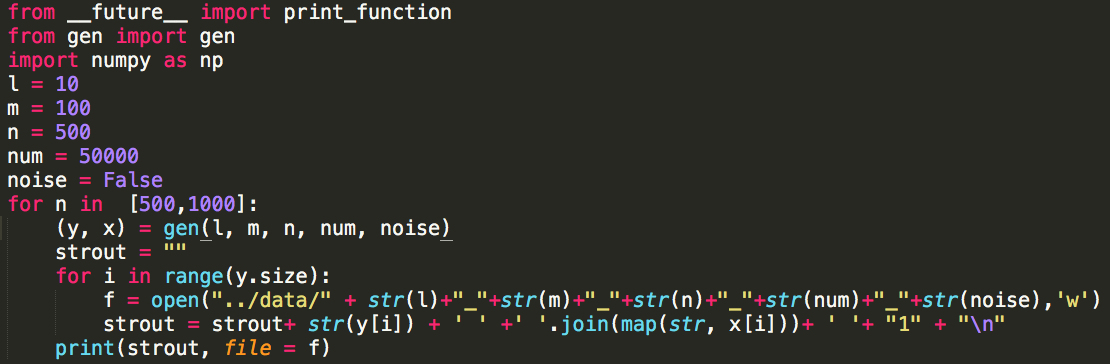
\includegraphics[width = 0.9\textwidth]{pythoncode.png}

\item[(b)]Parameters Tuning\\
1. For Perceptron, $\eta = 1$, $\gamma = 0$. Nothing needs to be swept.\\ 
2. For Perceptron w/margin, choose $\eta \in \{1.5,0.25,0.03,0.005,0.001\}$, $\gamma = 1$.\\ 
3. For Winnow, choose $\alpha \in \{1.1,1.01,1.005,1.0005,1.0001\}$, $\gamma = 0$.\\
4. For Winnow w/margin, choose $\alpha \in \{1.1,1.01,1.005,1.0005,1.0001\}$, \\$\gamma \in \{2.0,0.3,0.04,0.006,0.001\}$.\\
5. For AdaGrad, choose $\eta \in \{1.5,0.25,0.03,0.005,0.001\}$, $\gamma = 1$.
  \begin{center}
    \begin{tabular}{|p{2.2cm}|p{6cm}|p{6cm}|}
      \hline
      Algorithm  &  Dataset n=500 & Dataset n=1000\\\hline\hline
      Perceptron &  Accu = 0.9718 &   Accu = 0.9504\\\hline
      Perceptron w/margin & $\eta=0.005$, Accu = 0.9868 & $\eta=0.03$, Accu = 0.9574\\\hline
      Winnow   & $\alpha=1.1$, Accu = 0.9958 & $\alpha=1.1$, Accu = 0.9954 \\\hline
      Winnow w/margin   & $\alpha=1.1$, $\gamma=2$, Accu = 0.9994 & $\alpha=1.1$, $\gamma=2$, Accu = 0.997 \\\hline
      AdaGrad  & $\eta=0.25$, Accu = 0.9994 & $\eta=0.25$, Accu = 0.997 \\\hline
    \end{tabular}
  \end{center}
Then, use the parameters get for the experiment above to gather accumulated error times. Recording the total error times for each 100 training examples. Plot the result for 5 algorithm. X axis means the number of training examples and Y axis means the accumulated error times.\\
\clearpage
\begin{center}
\begin{figure}%
  \begin{subfigure}{0.49\textwidth}
    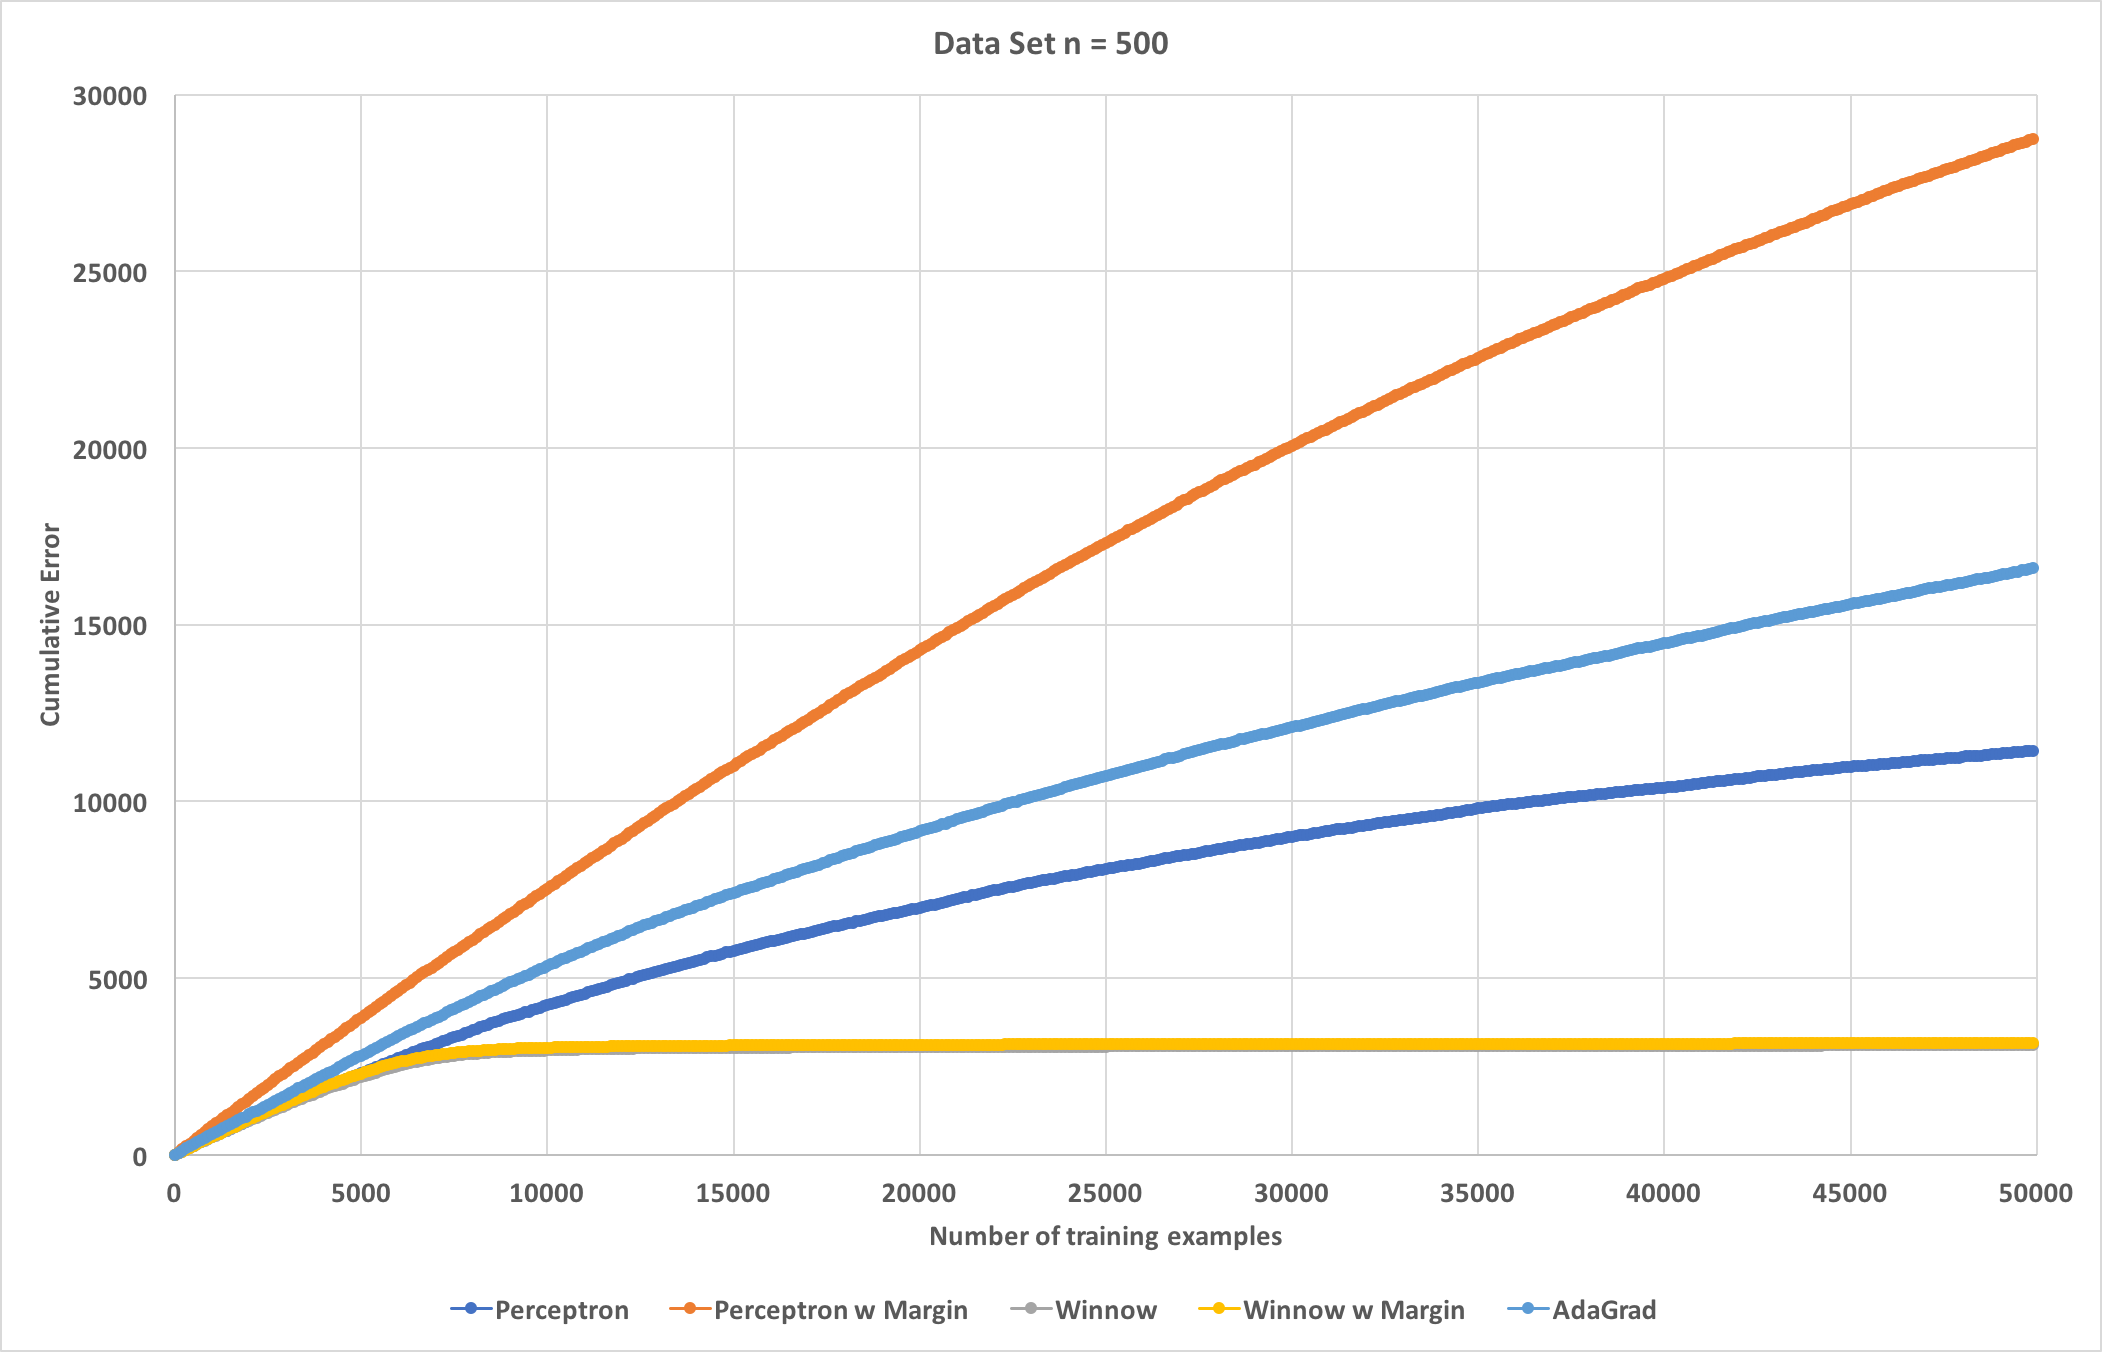
\includegraphics[width = \textwidth]{n500.png}
    \caption{Number of training examples vs Cumulative Error, Dataset n = 500}
    \label{fig:left}
  \end{subfigure}
  \begin{subfigure}{0.49\textwidth}
    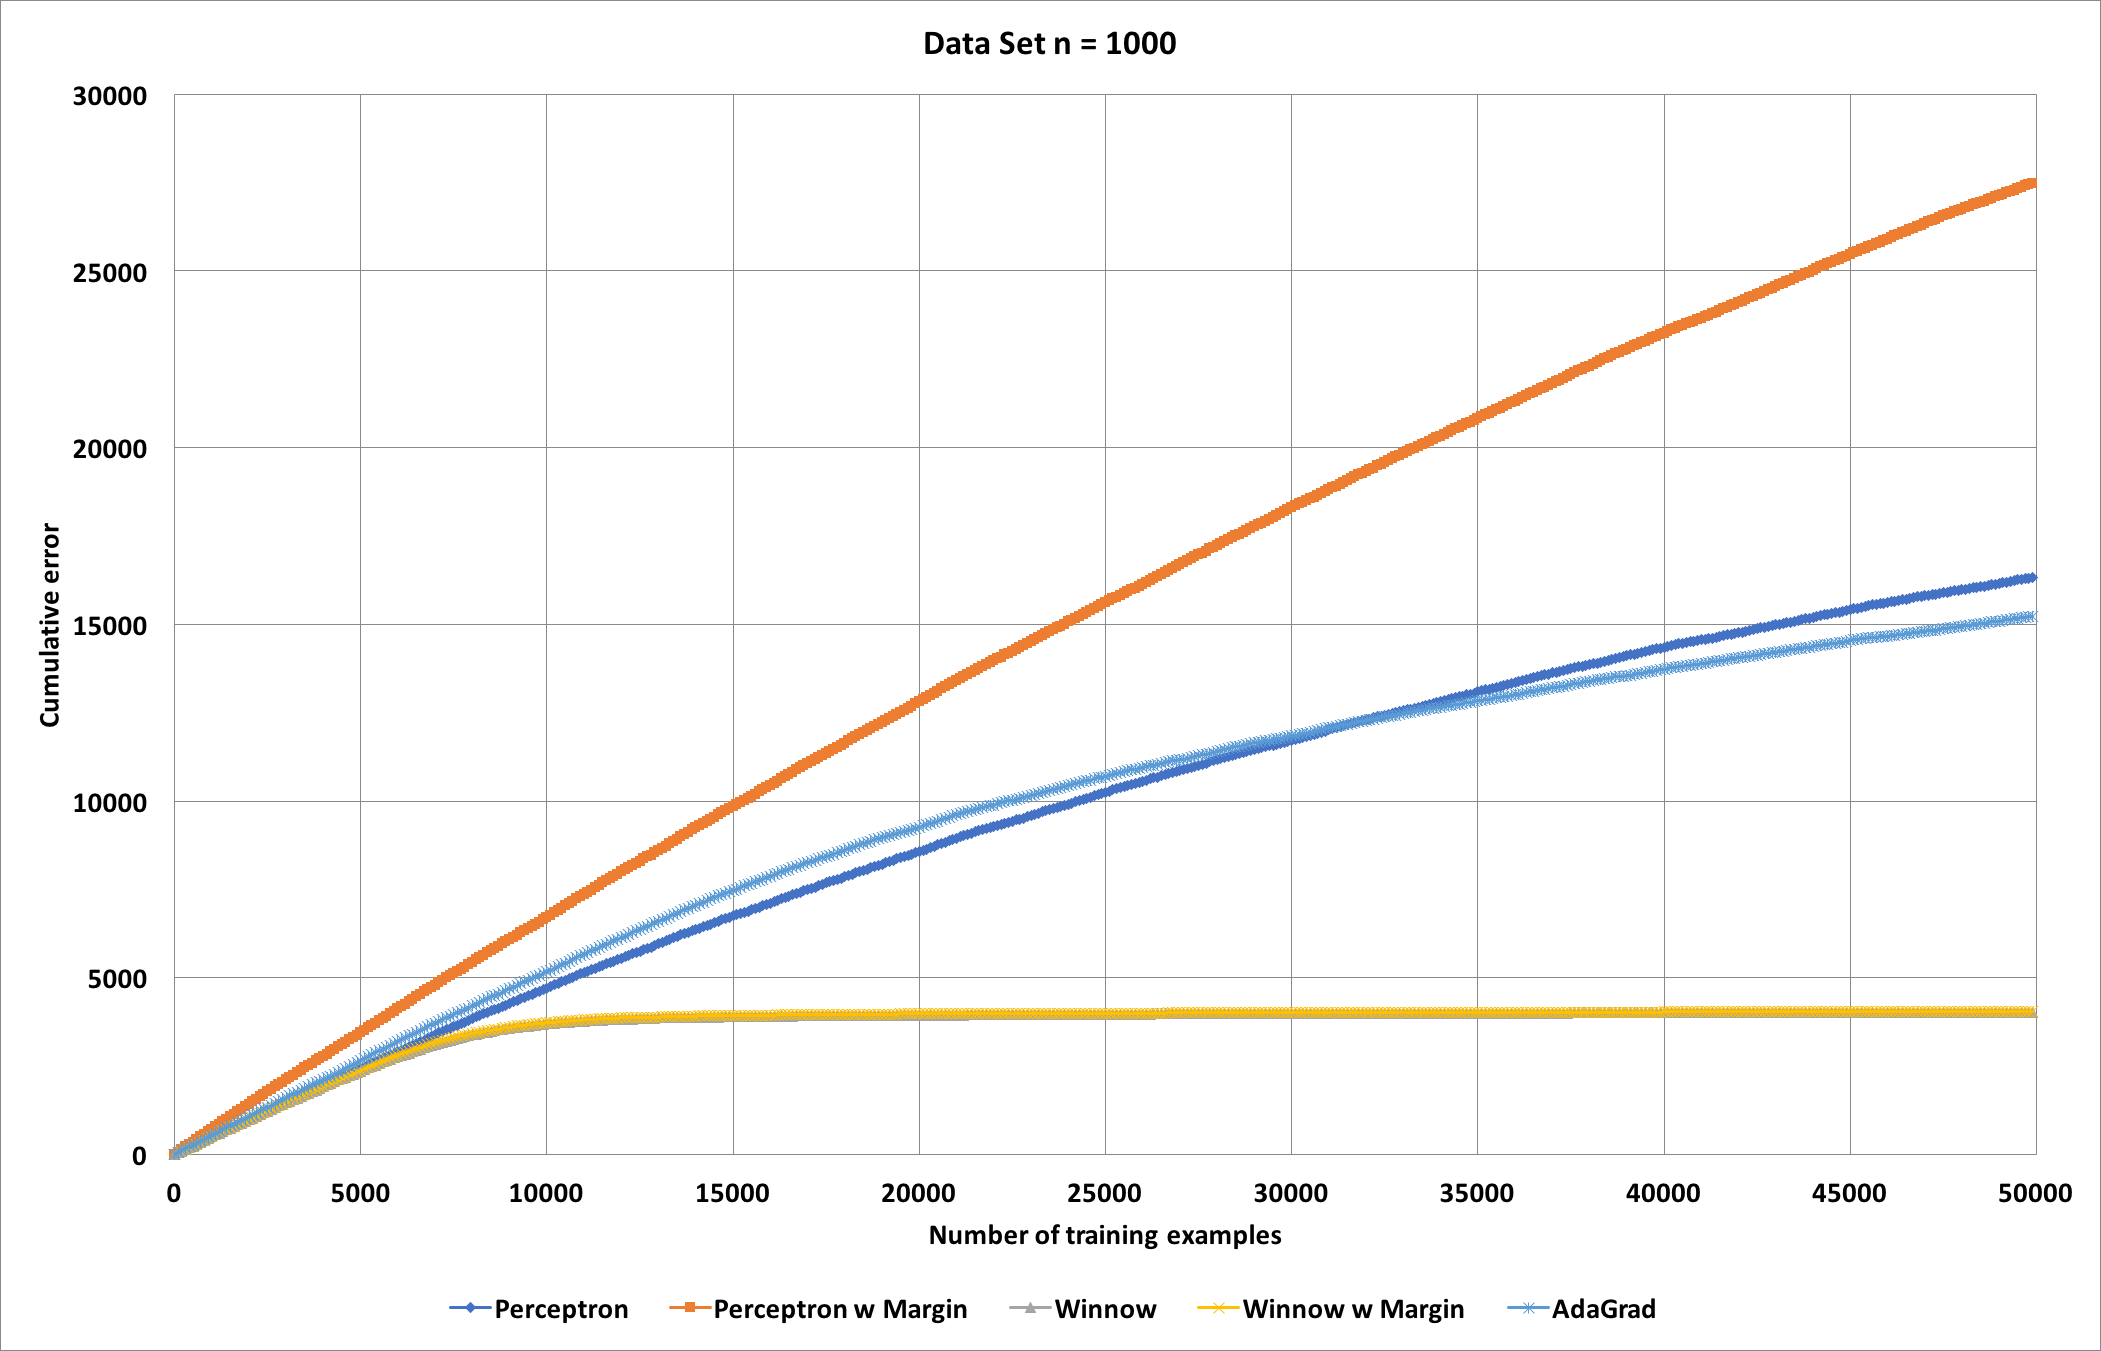
\includegraphics[width = \textwidth]{n1000.png}
    \caption{Number of training examples vs Cumulative Error, Dataset n = 1000}
    \label{fig:right}
  \end{subfigure}
\end{figure}
\end{center}
For Perceptron, the increase of $\gamma$ will take more times to learn the weight vector.  
For Winnow, the algorithm adjusts the weight vector using exponential coefficient faster than others and has no apparent affect by the n of the dataset.
For AdaGrad, it works like Perceptron due to the similarity of the curves. With n = 1000 dataset, performance of AdaGrad is better than Perceptron. That implies AdaGrad is doing better in sparse data.  